\begin{surferIntroPage}{Singularitats simples}{simplesing_A1pm}{Singularitats simples}
Es diu que una superfície és \emph{llisa} o \emph{no singular}
si, en termes intuïtius, no té punxes, arestes o plecs
(aquesta mena de punts especials es diu que són
\emph{singulars}). Les dues primeres imatges, l'esfera i el tor,
són exemples de superfícies llises:
    \begin{center}
      \vspace{-0.2cm}
      \begin{tabular}{@{}c@{}c@{}c@{\quad}c@{}c@{}c@{}c@{}}
        \begin{tabular}{@{}c@{}}
          Llises:
        \end{tabular}
        &
        \begin{tabular}{@{}c@{}}
          \includegraphics[width=1.1cm]{../../common/images/kugel}
        \end{tabular}
        &
        \begin{tabular}{@{}c@{}}
          \includegraphics[width=1.1cm]{../../common/images/torus}
        \end{tabular}
        &
        \begin{tabular}{@{}c@{}}
          Singulars:
        \end{tabular}
        &
        \begin{tabular}{c@{}@{}}
          \includegraphics[width=1.1cm]{../../common/images/kegel}
        \end{tabular}
        &
        \begin{tabular}{c@{}@{}}
          
\includegraphics[width=1.1cm]{../../common/images/A2pm}
        \end{tabular}
        &
        \begin{tabular}{c@{}@{}}
          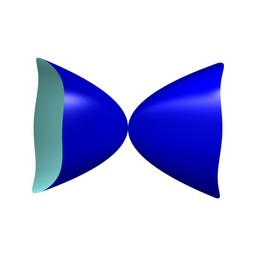
\includegraphics[width=1.1cm]{../../common/images/A3pm_0}
        \end{tabular}
      \end{tabular}
    \end{center}
    \vspace{-0.2cm}
Les singularitats més simples són conegudes com a \emph{ADE}, com
ara les del tipus
$A_k^{\pm\pm}$, definit per l'equació
    $x^{k+1}\pm y^2\pm z^2=0$.
La superfície blava de la imatge, té un punt singular de tipus
$A_3^{+-}$, la magenta, de tipus
$A_2^{+-}$, i la de color roig (el \emph{con quadràtic}),
de tipus $A_1^{+-}$.
Les singularitats ADE tenen relacions sorprenents, encara no ben
enteses, amb nombroses branques de les matemàtiques i la física, i amb
la natura. Cada $A_k$
es pot deformar en $\lfloor\frac{k+1}{2}\rfloor$
singularitats $A_1$; d'una
$A_3^{+-}$, s'obtenen dues $A_1^{+-}$ (imatges dessota a
l'esquerra):
%\vspace*{-3pt}
%    \dontshow{
    %
    \begin{center}
      \vspace{-0.2cm}
      \begin{tabular}{@{}c@{\quad}c@{}c@{\qquad\quad}c@{\quad}c@{\quad}c@{}}
        \begin{tabular}{@{}c@{}}
          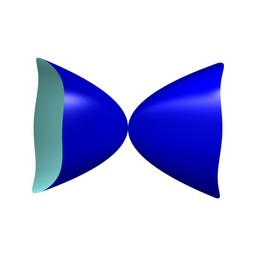
\includegraphics[width=1.2cm]{../../common/images/A3pm_0}
        \end{tabular}
        &
        \begin{tabular}{@{}c@{}}
          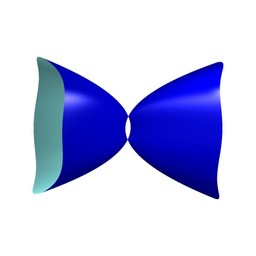
\includegraphics[width=1.2cm]{../../common/images/A3pm_1}
        \end{tabular}
        &
        \begin{tabular}{@{}c@{}}
          
\includegraphics[width=1.2cm]{../../common/images/A3pm_2}
        \end{tabular}
        &
        \begin{tabular}{@{}c@{}}
          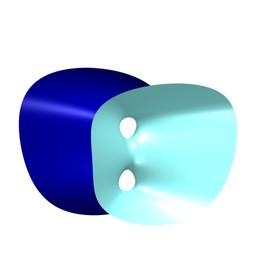
\includegraphics[width=1.2cm]{../../common/images/A3pm_vz_2}
        \end{tabular}
        &
        \begin{tabular}{@{}c@{}}
          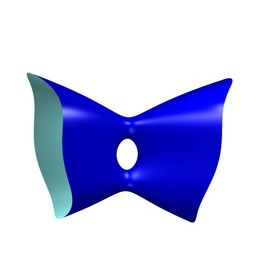
\includegraphics[width=1.2cm]{../../common/images/A3pm_vz_1}
        \end{tabular}
        &
        \begin{tabular}{@{}c@{}}
          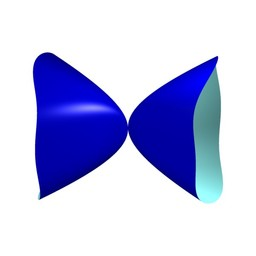
\includegraphics[width=1.2cm]{../../common/images/A3pm_vz_0}
        \end{tabular}
      \end{tabular}
      \\
      \begin{tabular}{@{}c@{\qquad\qquad}c@{}}
          $A_3 \qquad\quad \rightarrow \qquad 2 A_1$
          &
          $2$ cicle $+$ $1$ cicle \ $\rightarrow \ A_3$
        \end{tabular}
    \end{center}
%    }
    \vspace*{-0.2cm}
L'índex $k$ de $A_k$ és l'anomenat
\emph{nombre de Milnor}: és el nombre de
\emph{cicles evanescents} de la singularitat, això és, el nombre de
forats que desapareixen quan es contrauen en el punt singular
(vegeu les tres imatges a la dreta).
 
\end{surferIntroPage}
